\section{Data Analysis}
Wrapping around the plug-in model of our system there are some auxiliary
software (scripts)
which follow and automate all the simulations, from the beginning (building up
the simulation scenario) to the post-processing data analysis.

Thus, after a bunch of simulation runs handled as previously explained,
 we performed a data analysis in order to
figure out the effectiveness of a time analysis attack.  

In this section we will illustrate the software tools we used for
handling the
simulation runs and the software tools we used in the analysis phase. 
Eventually we will 
present the empirical results
obtained.
\subsection{Netbuilder and Launcher Scripts}
As described in \ref{sec:Shadow}
The Shadow simulator use a XML file to describe the network,
we automatize this process with a python script called the net-builder script.\\
This script will so build a scenario based on some input parameters as:
\begin{itemize}
\item The number of TOR relays in the simulation.
\item The number of TOR exit nodes in the simulation.
\item The number of TOR 4authorities\footnote{A 4 Authority node is simply the
database that keep track of the state of the TOR network and the list
of the TOR relays/exit-nodes} nodes in the simulation.
\item The number of clients (simpletcp) of the simulation.
\item The number of servers (simpletcp) of the simulation.
\item The percentage of clients tracked by an autosys plug-in.
\item The percentage of servers tracked by an autosys plug-in.
\item The density of the network-requests.
\end{itemize}

When the others parameters are self-esplicative, the density parameter is somewhat
that deserves more that two words on.
This parameter specify the time interval between every connection made from the
simpletcp plug-in to emulate the behaviour of different type of networks.
We defined three behaviours to our network study:

\begin{itemize}
\item Slow:\\minimum: a mean of 800 milliseconds of sleep time between every connection,\\
            maximum: a mean of 2 seconds of sleep time between every connection.
\item Average:\\minimum: a mean of 80 milliseconds of sleep time between every connection,\\
               maximum: a mean of 1 second of sleep time between every connection.
\item Fast:\\minimum: a mean of 20 milliseconds of sleep time between every connection\\
            maximum: a mean of 100 milliseconds of sleep time between every connection.
\end{itemize}

This normal distributed values are computed for every simpletcp client
(which will compute a random uniform distributed value as described in \ref{sec:simpletcpclient}).\\

The second auxiliary script we used is a bash script that helped us in the
automatic run of the simulations.
This script will run a bunch of simulation using the algorithm \ref{alg:launcher}.

\begin{algorithm}[H]
\caption{Launcher script}
\begin{algorithmic}[2]
\For{($simulation\_run \gets 1$; $simulation\_run <= steps$; $simulation\_run++$)}
	\For{($sim\_id \gets 1$; $sim\_id <= simulations\_per\_step$; $sim\_id++$)}
		\ForAll {$density$ $in$ $(slow, fast, average)$}
		\If {The client trace percentage is not fixed}
			\State $client\_trace\_value \gets sim\_id/simulations\_per\_step$
		\EndIf
		\If {The server trace percentage is not fixed}
			\State $server\_trace\_value \gets sim\_id/simulations\_per\_step$
		\EndIf
		\If{A configuration is present for $<sim\_id, density>$ And the percentages are fixed}
			\State Use the previous configuration
		\Else
			\State Generate a new configuration with net-builder
		\EndIf
		\State Launch the Shadow Simulator with the appropriate configuration.
		\EndFor
	\EndFor
\EndFor
\end{algorithmic}
\label{alg:launcher}
\end{algorithm}

From this algorithm we can see that we can use this script to create a set of
simulations with some linear modifications to the numbers of the traced clients
or the number of the traced servers (or a combination of the two).
We can also declare more than one run on this bunch of simulations, this can
be useful to compute the mean values from the same configuration file, else we
can generate a new configuration file starting from some input parameters.

After the launch we can pass the simulation raw data to the analyzer script.

\subsection{Analyzer Script}
The analyzer script takes a log file, generated previously by the logger
server, as input and tries to
ascertain which clients were communicating with which server during the
simulation. The log file is a list of entries that are formatted as described in
 figure \ref{fig:analyzer_pack_struct} and the figure
\ref{fig:example_log_file} shows an example of it.
\begin{figure}[H]
\centering
\begin{lstlisting}[language=bash,frame=single, numbers=left]
...
c;client10;1420000000
s;server7;1420008031
c;client6;1420005867
s;server9;1420146660
s;server6;1420205384
s;server8;1420252482
c;client0;1420680882
c;client1;1421017740
s;server7;1421023888
s;server2;1421156205
c;client8;1421160529
s;server3;1421318345
s;server0;1421332488
c;client7;1421487295
c;client4;1421634744
s;server9;1421726485
c;client2;1421827747
...
\end{lstlisting}
\caption{Analyzer log file fragment example.}
\label{fig:example_log_file}
\end{figure}
The script scans the log file and for each line checks whatever the entry is
related to a client or a server. If the entry refers to a client
connection request it scans in a nestled loop the server connection entries
that may be related to that client. The nested loop does not scan the whole
file until its end, but it stops after a sufficient amount of
read entries. In particular, the amount of entries to be read is
measured in time: from a client entry, the scan goes
ahead until the difference between the time-stamp of the current scanned 
entry and the time-stamp of the starting client entry is not greater
than a fixed threshold $thr_{max}$. For our experiment we chose a limit of 6
seconds as it is an enough high latency
value for a connection acceptance. Likely, the average latency for a
connection response, even passing through the Tor network, is
considerably smaller than 6 seconds but anyway we can over-esteem a bit this
value without unexpected bad consequences. On the other hand, an under-esteem of
this value would threaten the analysis results. 

Furthermore, from a client
entry the nestled scan starts reading from the entry that is 100 ms far
from the client start point. This lower threshold, $thr_{min}$, is needed in order to
 filter those server entries that registered a connection time-stamp
that results too young for being related to the client start point. This
lower limit is more critical: a too low limit would guarantee false
positive results and a too high limit would drop the right results.
We will see later that after some tests, a value around 100ms seemed to maximize 
the clients servers relation matching. %TODO in empirical results

The analysis proceeds by recording a set of possible server candidates 
 per each client connection request. Each server candidate $s$ assumes a
$pmatch(creq,s)$ value which
indicates how much a server candidate can be the real
\footnote{The term ''real`` should not be misunderstood with
non-simulated but should be intended as non-estimated.}
 server that
accepted the $creq$
client request. The $pmatch$ value is defined
as following:
\begin{equation}
pmatch(creq, s) = 1 - \frac{\Delta_t(creq, s) - thr_{min}}{thr_{max} - thr_{min}}
\end{equation}
where $\Delta_t(creq, s)$ is the time distance between the entry
time-stamp of the server $s$ related to the entry time-stamp of the client connection request
$creq$.

As instance let us consider the server candidates related to the first
client entry, $client10$, of the example log
fragment shown in figure \ref{fig:example_log_file}: 
$server7$ is not considered at all in the $pmatch$ calculation  as
$\Delta_t$ 
is lesser than $thr_{min}$; then the $pmatch$ values for the first server
candidates related to the client request c;client10;1420000000 are shown in figure \ref{fig:pmatch}:
\begin{figure}[h]
\begin{lstlisting}[language=bash,frame=single, numbers=left]
candidate 	pmatch
server9 	0.992
server6 	0.982
server8 	0.975
server7  	0.846
server2  	0.823 
server3  	0.769
server0  	0.794
...
\end{lstlisting}
\caption{$pmatch$ values for server candidates related to $client10$}
\label{fig:pmatch}
\end{figure}

Clearly the $pmatch$ probability is higher when the server connection is
closer to $thr_{min}$ meaning that the likelihood of a server
candidate to be the real server for the related client decreases when
the server connection acceptance attempted far from 100ms. 

Another fact that may be considered in a time-analysis is that if a server accepts a
connection request from a client after a certain time $\Delta_t$, that
server will likely accept again another connection from the same client
after a time that is close to $\Delta_t$ if the Tor communication path is the same as
before\footnote{If the connections are going to the same server, the Tor
daemon could reuse the same old Tor communication path for a maximum
than 10 minutes\cite{tormanual}.}. 
Thus, as the $pmatch$ is defined as the $\Delta_t$ normalization, 
let us define the $gap$ average related to a
server $s$ that is a candidate for a client $c$ as follows:

%TODO gap
\begin{equation}
\label{eq:gap}
 gap_{AVG}(c,s) = \frac{\sum_{i=0}^{N(c,s)} | pmatch(creq_{i+1},s) -
pmatch(creq_{i},s)
|}{N(c,s)}
\end{equation}

where $N(c,s)$ is the number of $c$ connection requests that have been likely
accepted from $s$.


At the end of the scan phase, each client collects a set of server
candidates with their relative average $gap$ and $score$ that is defined
as follows:
\begin{equation}
	score(c,s) = \frac{\sum_{i=0}^{N(c,s)} pmatch(creq_{i},s)}{gap_{AVG}(c,s) + 1}
\end{equation}

After that every server candidate related to a certain client gained
their own score, they are sorted, in a descending order, by the score
itself. The first of the list is elected as the best candidate to be the
right server that accepted the connection requests from its corresponding
client.

Let us notice that a candidate score highly depends by the number of connection
acceptances estimated for that candidate as by as the $pmatch$ sum gained,
meaning that more connection acceptances of a server are close to the client
requests (plus the $thr_{min}$) more the score for that server is high.
Also, the score is highly attenuated by the $gap_{AVG}$ if the connection
latencies often differs between each-others.


The analyzer script also collects information about the
real connections logged by the simple-tcp applications. With this
information the analyzer can tell us how much the estimated results are
close to the real ones. Obviously, in a real time analysis attack the real connections
information cannot be obtain by the client and server applications themselves 
but in a simulation environment, we can better figure out how a real
time analysis attack may be effective.

Moreover by a set of simulations
that provide the use of the real connections logged data an attacker
may be able to understand the matching accuracy of the analysis, how distinguish the
matched servers among the others and also evaluate some
parameters like $thr_{min}$ and $thr_{max}$ before 
experimenting the attack in a real scenario. 
With this in mind, the script
calculates the $matched\_accuracy$, a parameter that indicates how much
the matching of the right server (those that correspond with the real
data) is correct in terms of identified
connections:

\begin{algorithm}[H]
\caption{Matching accuracy calculation}
\begin{algorithmic}
\State $matched \gets 0$
\ForAll {$c$ \textbf{in} $traced\_clients$}
	\State $accuracy_c \gets null$
	\State $realsv \gets GetRealServer(c)$ 
	{\footnotesize \Comment The server which $c$ connected to}
	\State $s \gets GetBestServer(c_{SERVER\_CANDIDATES})$
	\If {$s$ = $realsv$}
		\State $N \gets GetConnectionNumber(c, s) $ 
		{\footnotesize \Comment The number of traced connections between $c$ and $s$}
		\State $M \gets GetConnectionNumber(c, realsv)$ 
		{\footnotesize \Comment The number of real connections between $c$ and $s$}

		\State $accuracy_c \gets \frac{ MIN(M, N)}{MAX(M, N)}$
	\State \textbf{break}
	\EndIf
	\If {$accuracy_c$}
		\State $matched\_clients \gets matched\_clients + 1$
		\State $matched\_accuracy \gets matched\_accuracy + accuracy_c$
	\EndIf	
\EndFor

\State $matched\_accuracy \gets matched\_accuracy / matched\_clients$
\State $matched\_portion \gets matched\_clients / traced\_clients$

\end{algorithmic}
\label{alg:launcher}
\end{algorithm}
 
The $accuracy_c$ contribution is calculated as the distance between the 
amount of the estimated matched connections
and the amount of the real connections.
The last but not least parameter is the $matched\_portion$ that indicates
how many traced clients found their right server. 


In the next paragraph we will look in details both the
$matched\_accuracy$ and the
$matched\_portion$
results obtained in different situations in order to understand how a
time analysis attack can be effective.

\newpage
\subsection{Empirical Results}

In order to retrieve an interesting results set we decided to conduct
3 different simulation macro-bunches with the following characteristics:
\begin{enumerate}
	\item The number of traced clients was fixed to almost 100\% of the
network and the number of traced server was increasing by one to another
simulation starting from 0 and ending to the 100\% of the network.
	\item The number of traced servers was fixed to almost 100\% of the
network and the number of traced clients was increasing by one to another
simulation starting from 0 and ending to the 100\% of the network.
	\item Both numbers of traced clients and traced servers (traced
network portion) was increasing by one to another
simulation starting from 0 and ending to the 100\% of the network.
\end{enumerate}

Each macro-bunch was executed 4 times in order to understand the results
average and their errors. 
Also, for each of those simulation macro-bunches, 10 simulation sub-bunches were
launched in order to provide a sufficient granularity in the traced
entities escalation. Moreover for each sub-bunch 3 simulations were
executed with 3 different values of the connections density: \textbf{slow},
\textbf{average}, \textbf{fast}. 

\begin{figure}
	\begin{subfigure}{.5\textwidth}
		\centering
		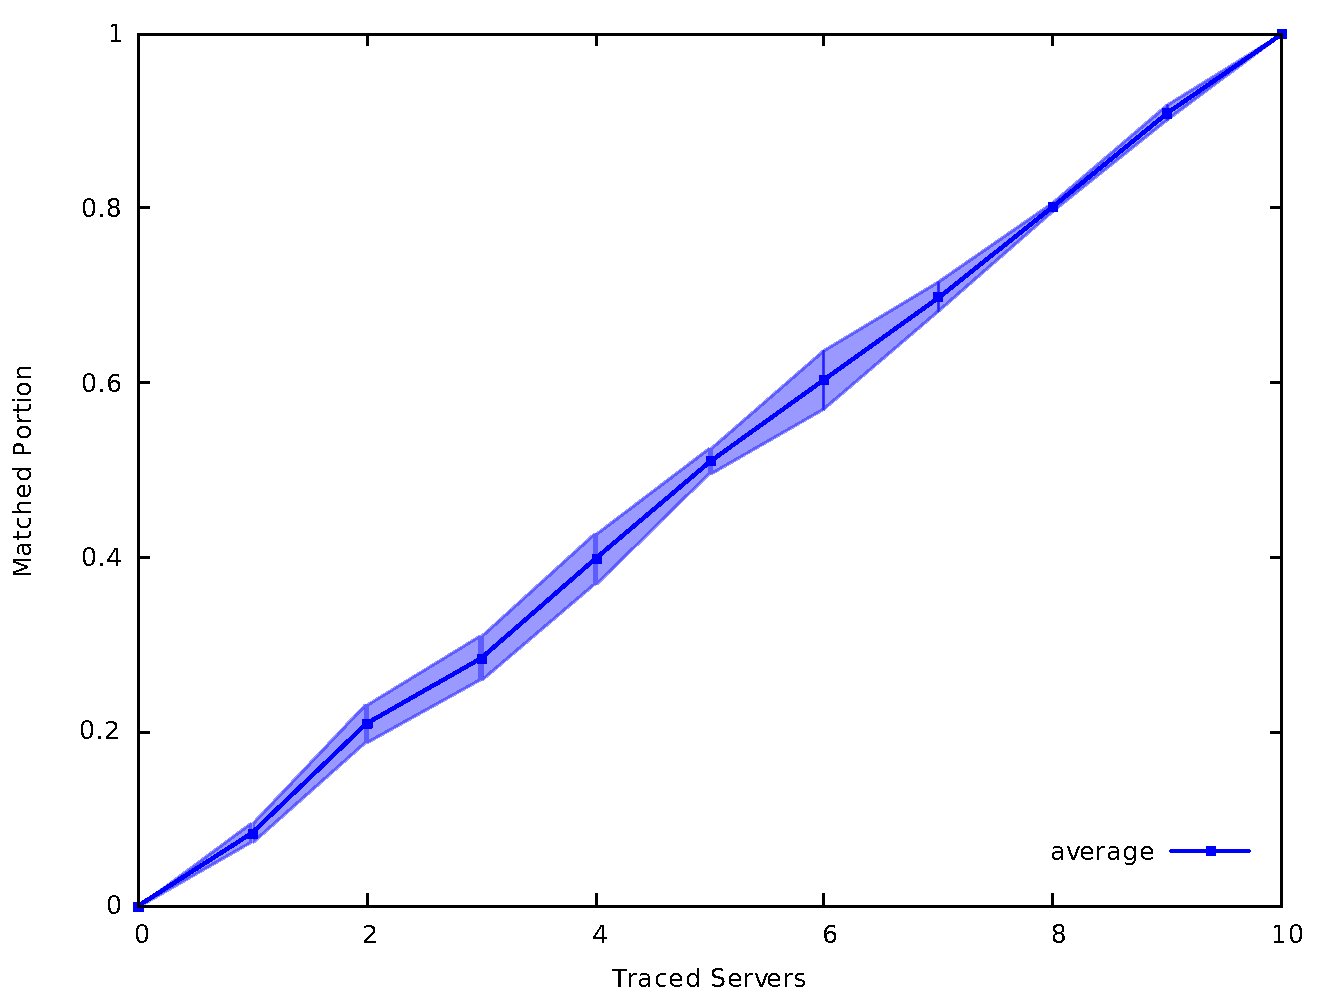
\includegraphics[width=1\linewidth]{graphs/s_server_mport_average_only.pdf}
		\caption{Matched portion related to the traced servers number}
		\label{fig:g_mporta}
	\end{subfigure} 
	\begin{subfigure}{.5\textwidth}
		\centering
		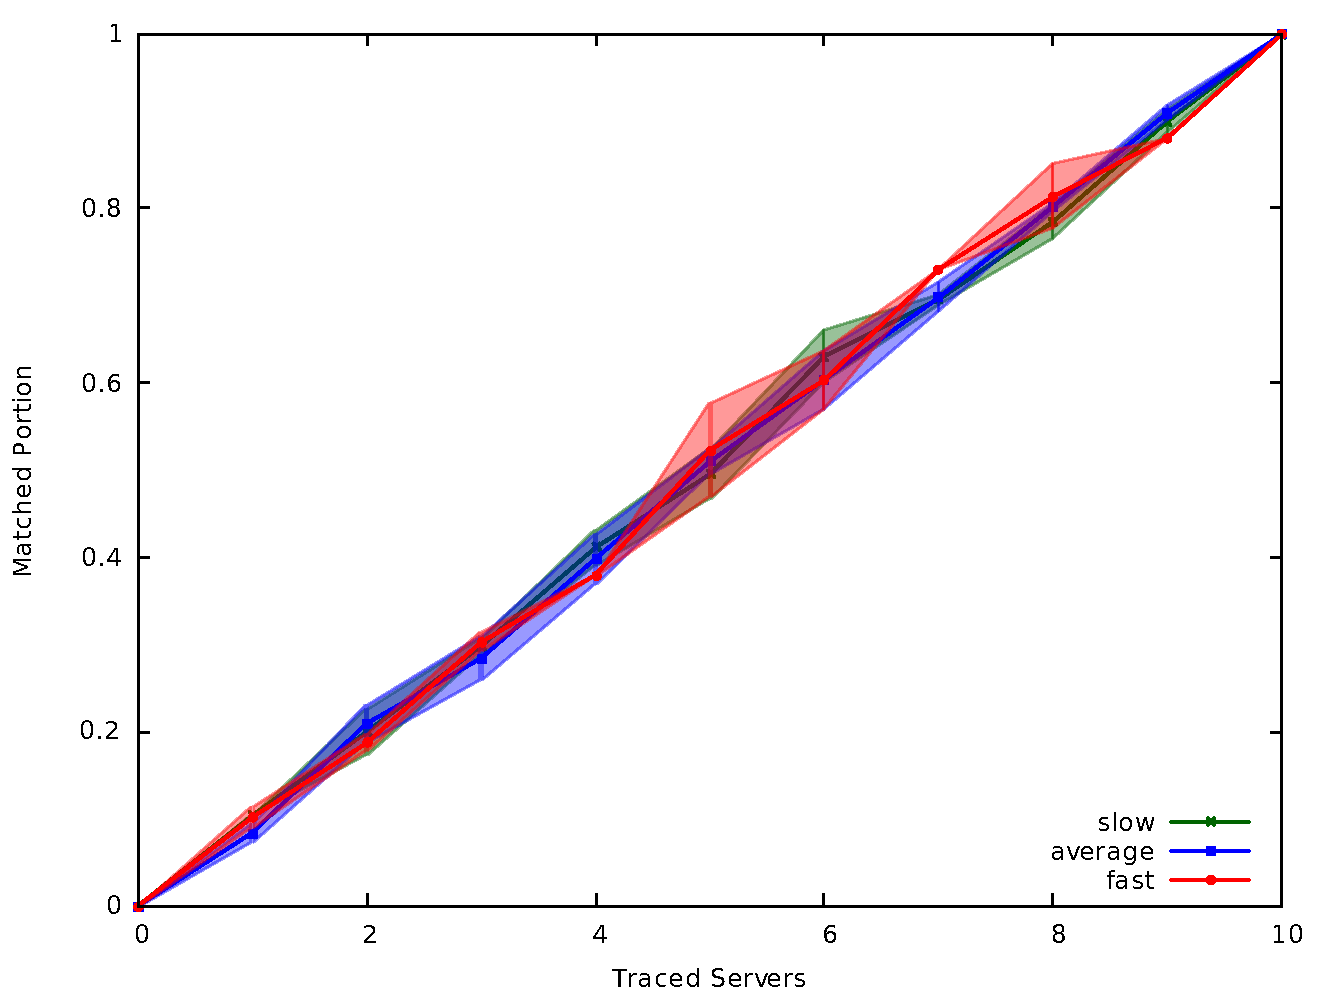
\includegraphics[width=1\linewidth]{graphs/s_server_mport.pdf}
		\caption{Same as frame $a$ but with different densities}
		\label{fig:g_mportb}
	\end{subfigure}

	\begin{subfigure}{.5\textwidth}
		\centering
		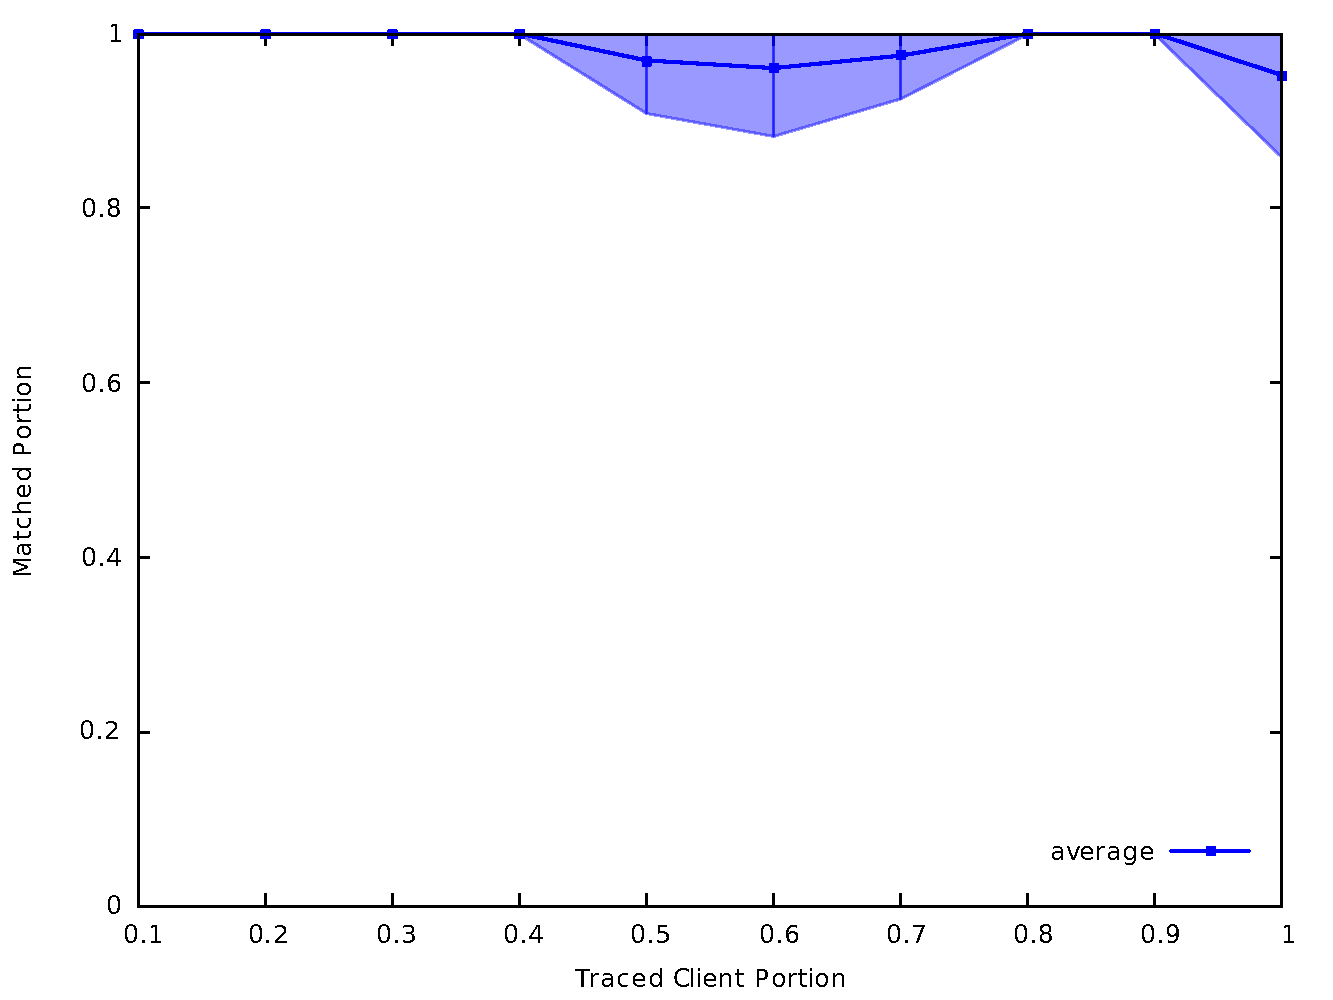
\includegraphics[width=1\linewidth]{graphs/c_tclient_mport_average_only.pdf}
		\caption{Matched portion related to the traced clients number}
		\label{fig:g_mportc}
	\end{subfigure}
	\begin{subfigure}{.5\textwidth}
		\centering
		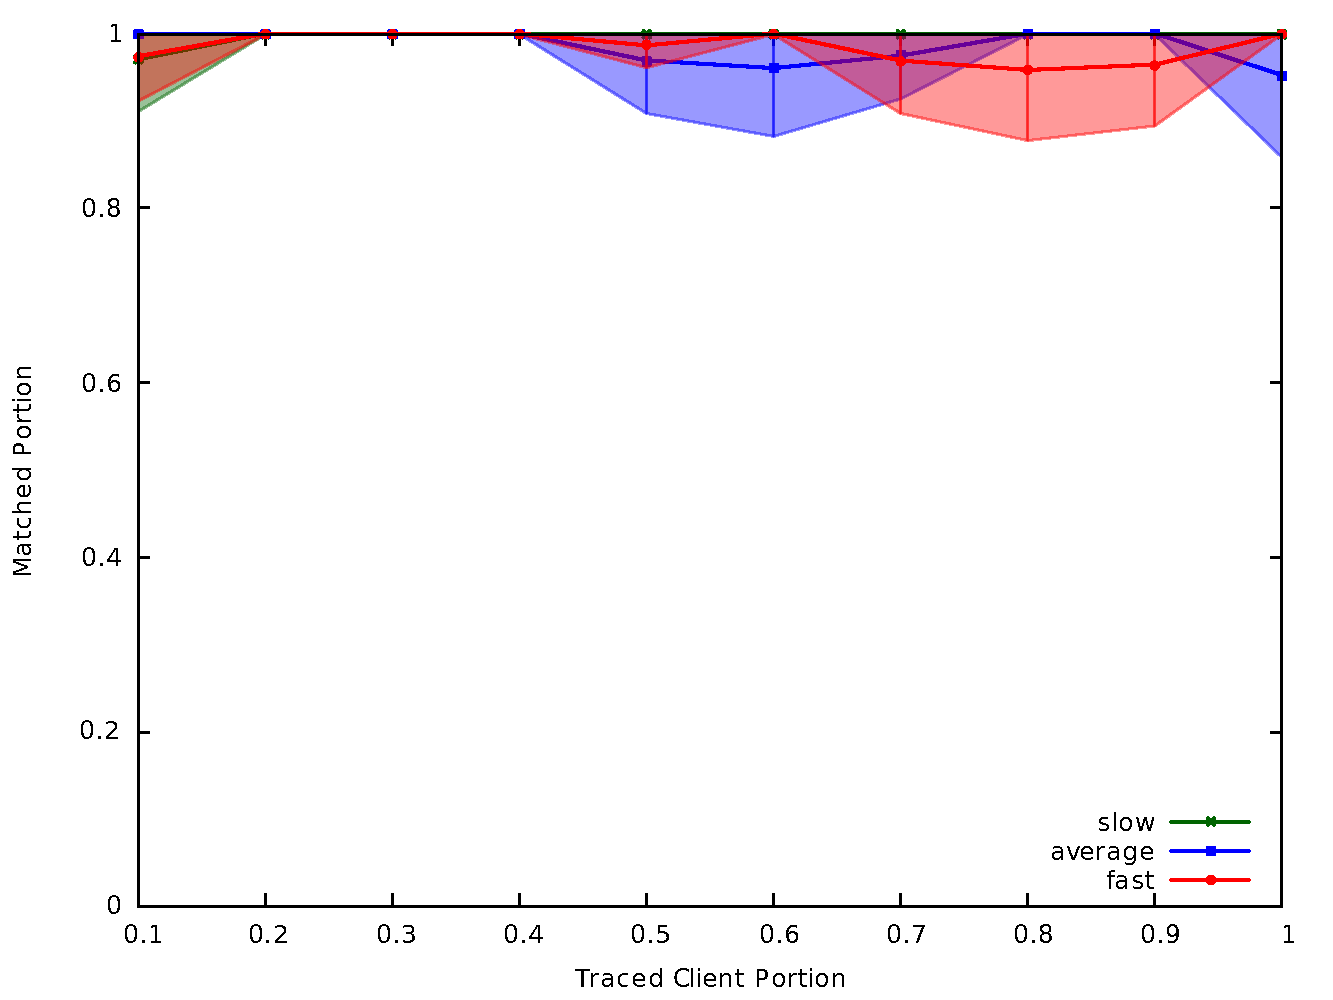
\includegraphics[width=1\linewidth]{graphs/c_tclient_mport.pdf}
		\caption{Same as frame $c$ but with different densities}
		\label{fig:g_mportd}
	\end{subfigure}

	\caption{Matched portion charts}
	\label{fig:g_mport}
\end{figure}

The figure set \ref{fig:g_mport} shows some charts about the matched
portion results. More specifically the figure \ref{fig:g_mporta}, shows
the test with the fixed number of traced clients and the variable number
of traced servers. As we can see the matched portion is almost linearly 
dependent by the number of traced servers.
This behavior was expected, in fact with a small amount of traced
servers most of the clients would not find their right server as its
connections are probably not logged. Also, it is interesting that
increasing the connections density (\ref{fig:g_mportb}) the function
trend seems to be more precise. This may be given by the fact that the
$gap_{AVG}$ tends to be more accurate increasing the number of
connections in the same temporal window, thus increasing the score of
the right
servers. Anyway it is comforting that while increasing the
connections density, the best candidate estimation does not seem to be affected by the 
 connections noise coming from the other server candidates.
Figures \ref{fig:g_mportc} and \ref{fig:g_mportd} show the experiments
with a fixed number of traced servers at 100\% and a variable number of
traced clients. We can see
that the matched portion tends to be constant around 80\% (as it was in
figure \ref{fig:g_mporta} with a hight portion of traced servers) at the variation of
the number of traced clients. This was also expected as the analysis is
conducted from the clients side (it searches the right servers of the
traced clients) and the matched portion is thus relative to the
number of traced clients. 

\begin{figure}
\begin{subfigure}{.5\textwidth}
		\centering
		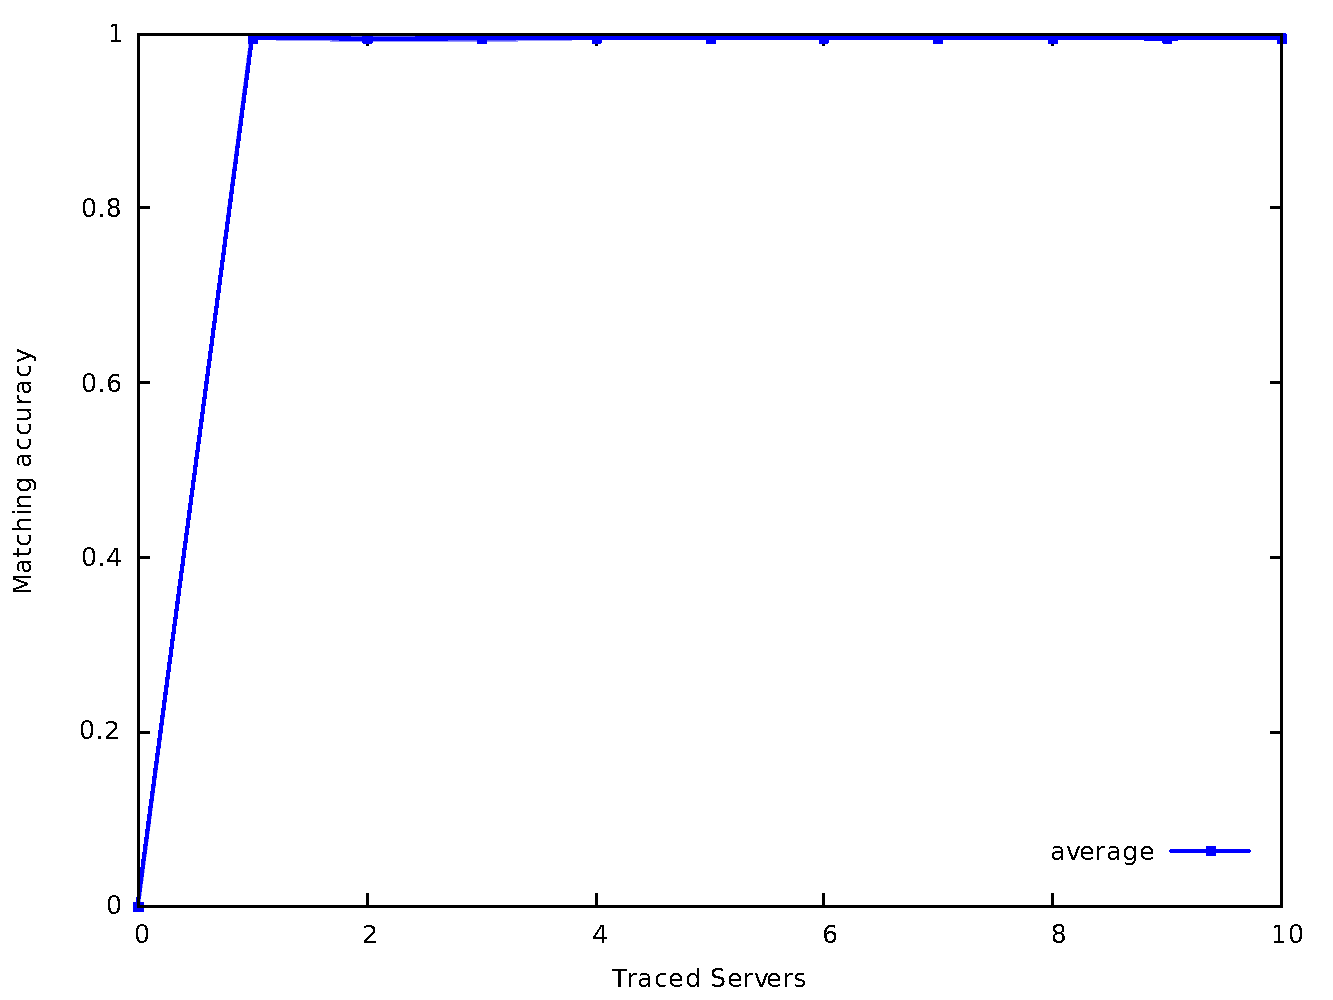
\includegraphics[width=1\linewidth]{graphs/s_server_pmatch_average_only.pdf}
		\caption{Matched accuracy related to the traced servers number}
		\label{fig:g_maccuracya}
	\end{subfigure} 
	\begin{subfigure}{.5\textwidth}
		\centering
		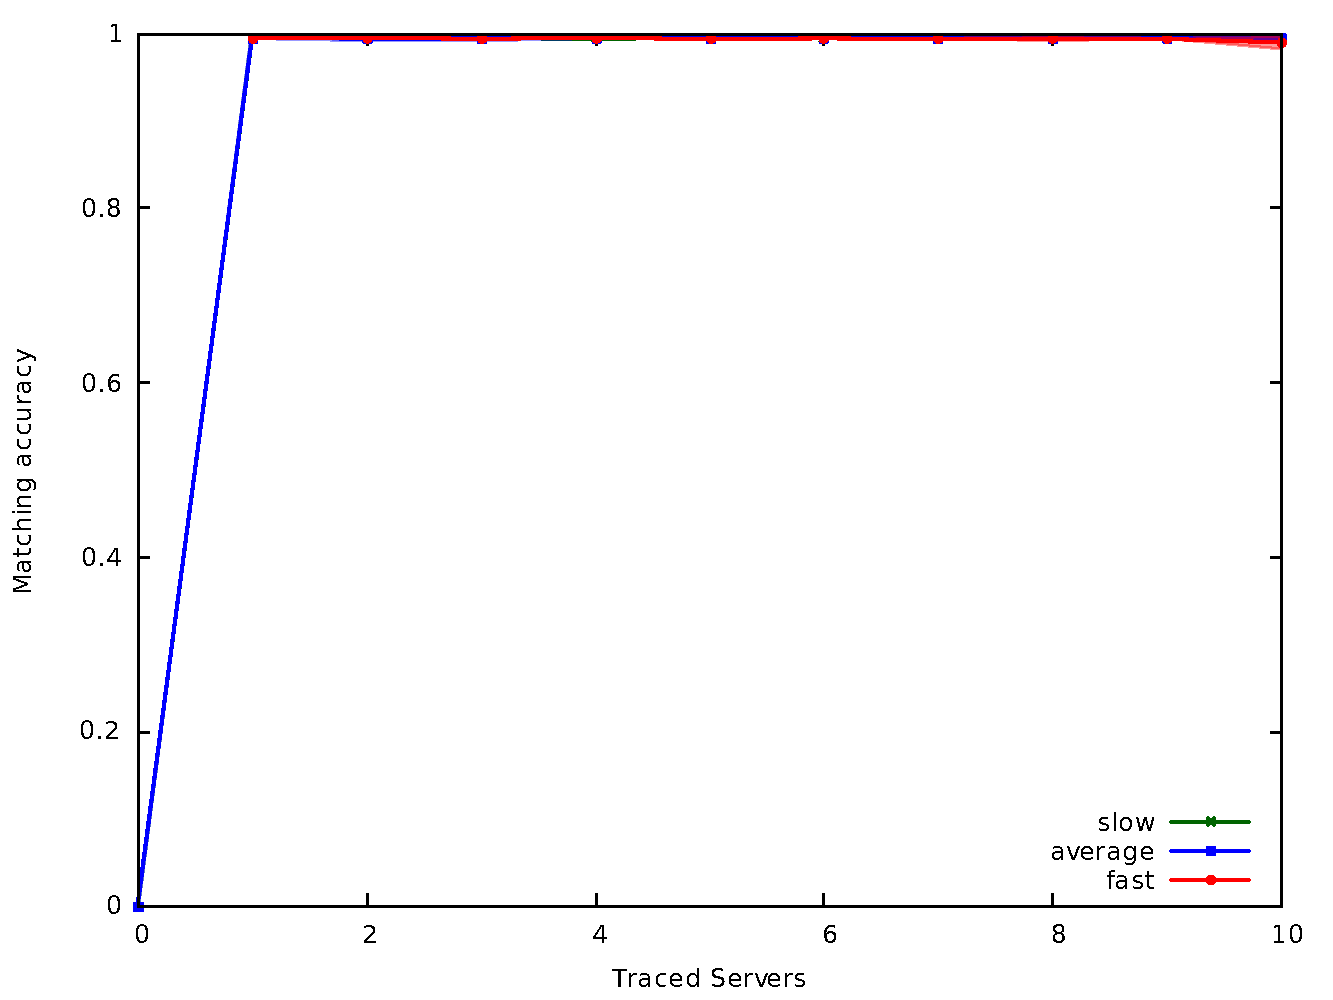
\includegraphics[width=1\linewidth]{graphs/s_server_pmatch.pdf}
		\caption{Same as frame $a$ but with different densities}
		\label{fig:g_maccuracyb}
	\end{subfigure}

	\begin{subfigure}{.5\textwidth}
		\centering
		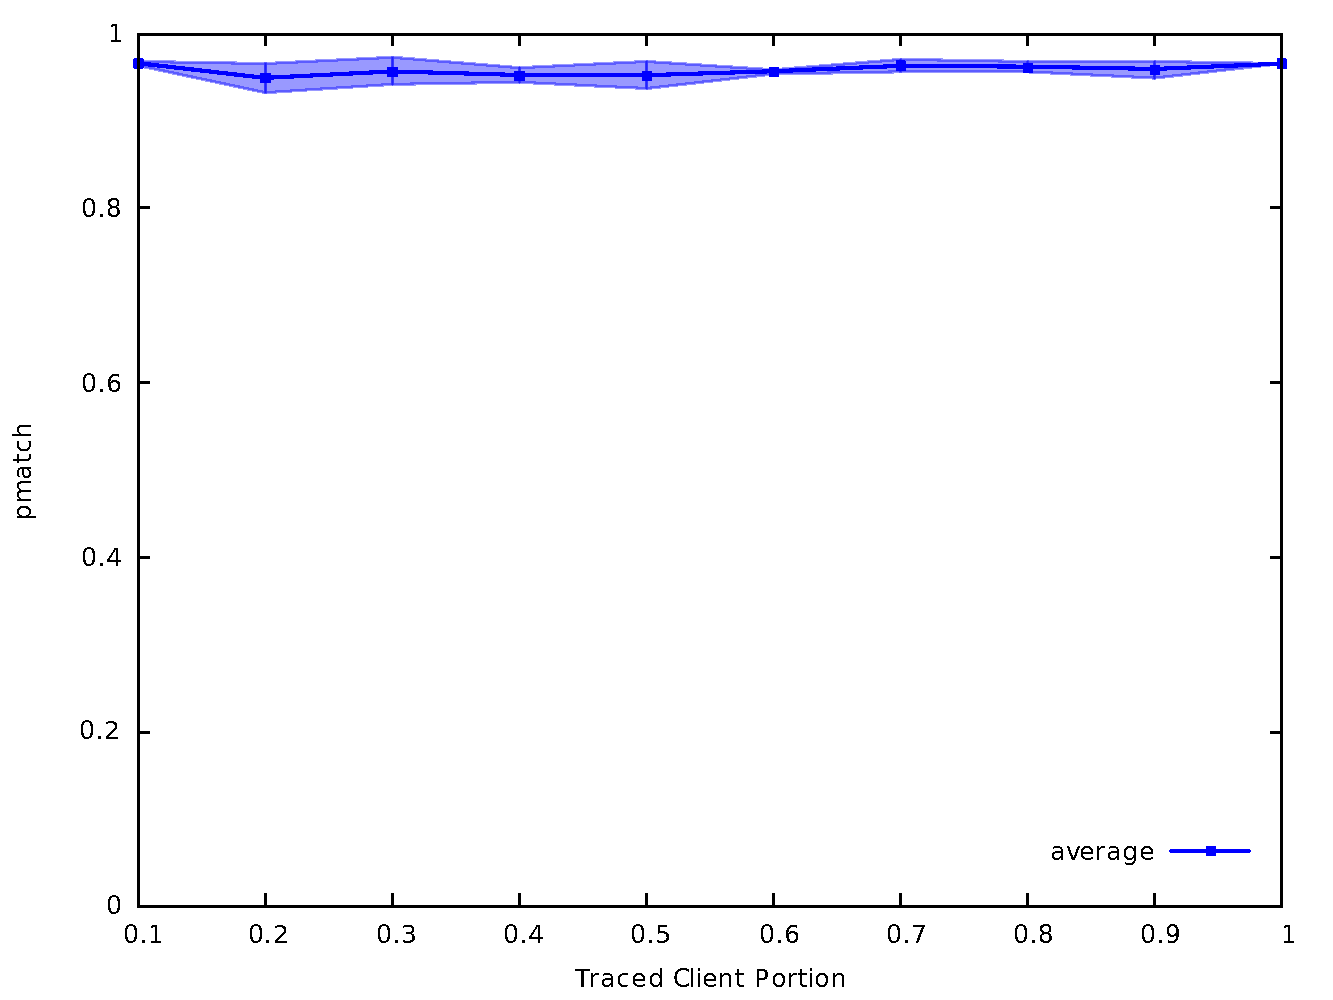
\includegraphics[width=1\linewidth]{graphs/c_tclient_pmatch_average_only.pdf}
		\caption{Matched accuracy related to the traced clients number}
		\label{fig:g_maccuracyc}
	\end{subfigure}
	\begin{subfigure}{.5\textwidth}
		\centering
		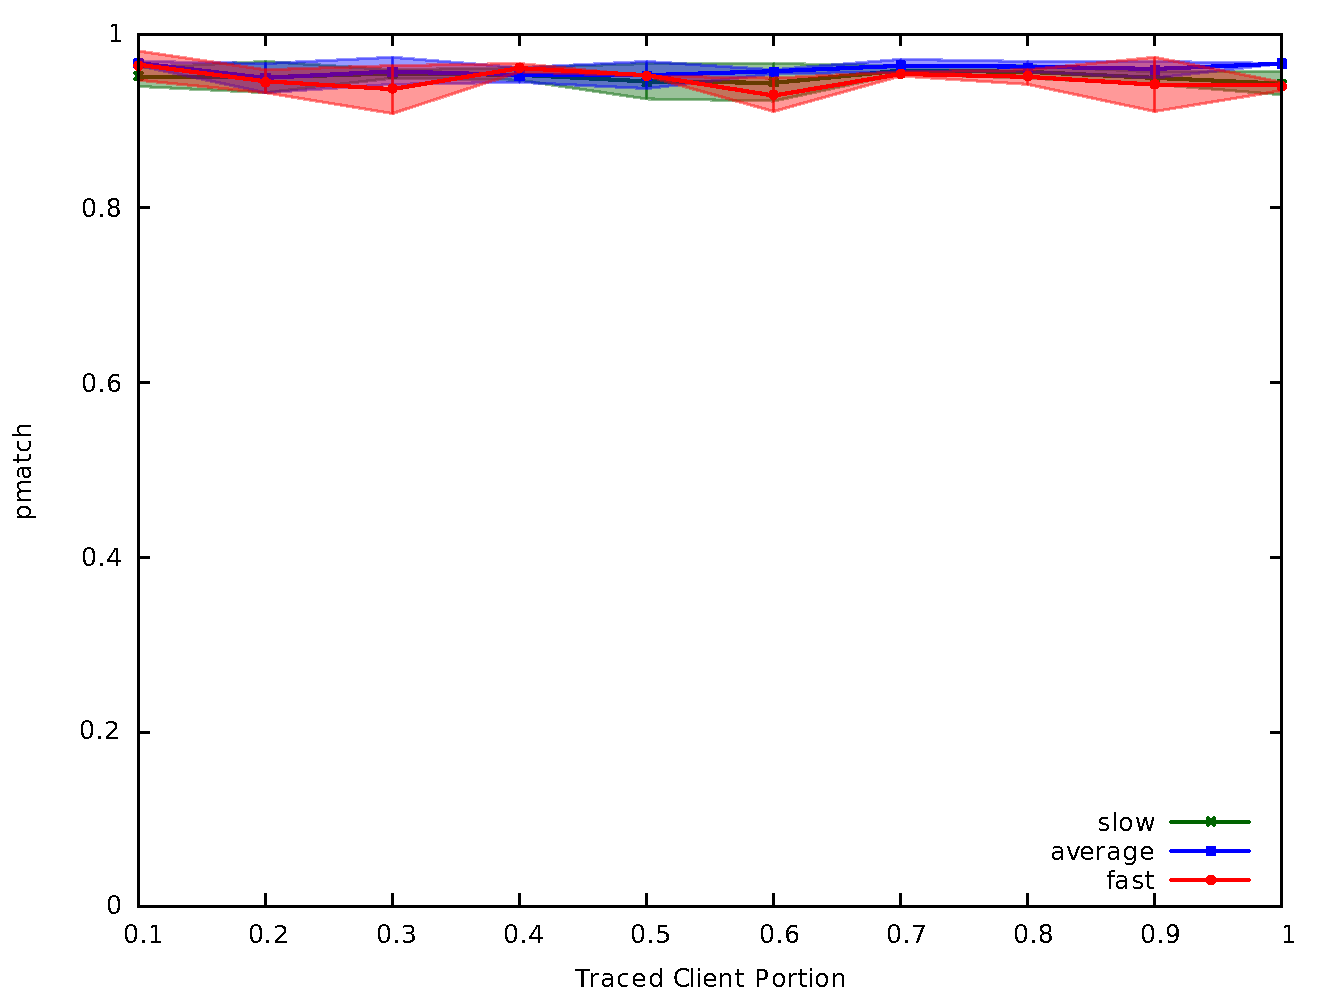
\includegraphics[width=1\linewidth]{graphs/c_tclient_pmatch.pdf}
		\caption{Same as frame $c$ but with different densities}
		\label{fig:g_maccuracyd}
	\end{subfigure}

	\caption{Matched accuracy charts}
	\label{fig:g_maccuracy}
\end{figure}

The charts shown in figure \ref{fig:g_maccuracy} shows the matching
accuracy results in the same order of the matched portion experiment
shown in figure \ref{fig:g_mport}. Clearly the matched accuracy is
almost constant around its maximum value, meaning that the clients who
correctly found their best candidates matched almost all the connections
from those servers. Moreover the matching accuracy does not
depend from any of the factors considered: traced clients number, traced
servers number and connections density.

\begin{figure}
	\begin{subfigure}{.5\textwidth}
		\centering
		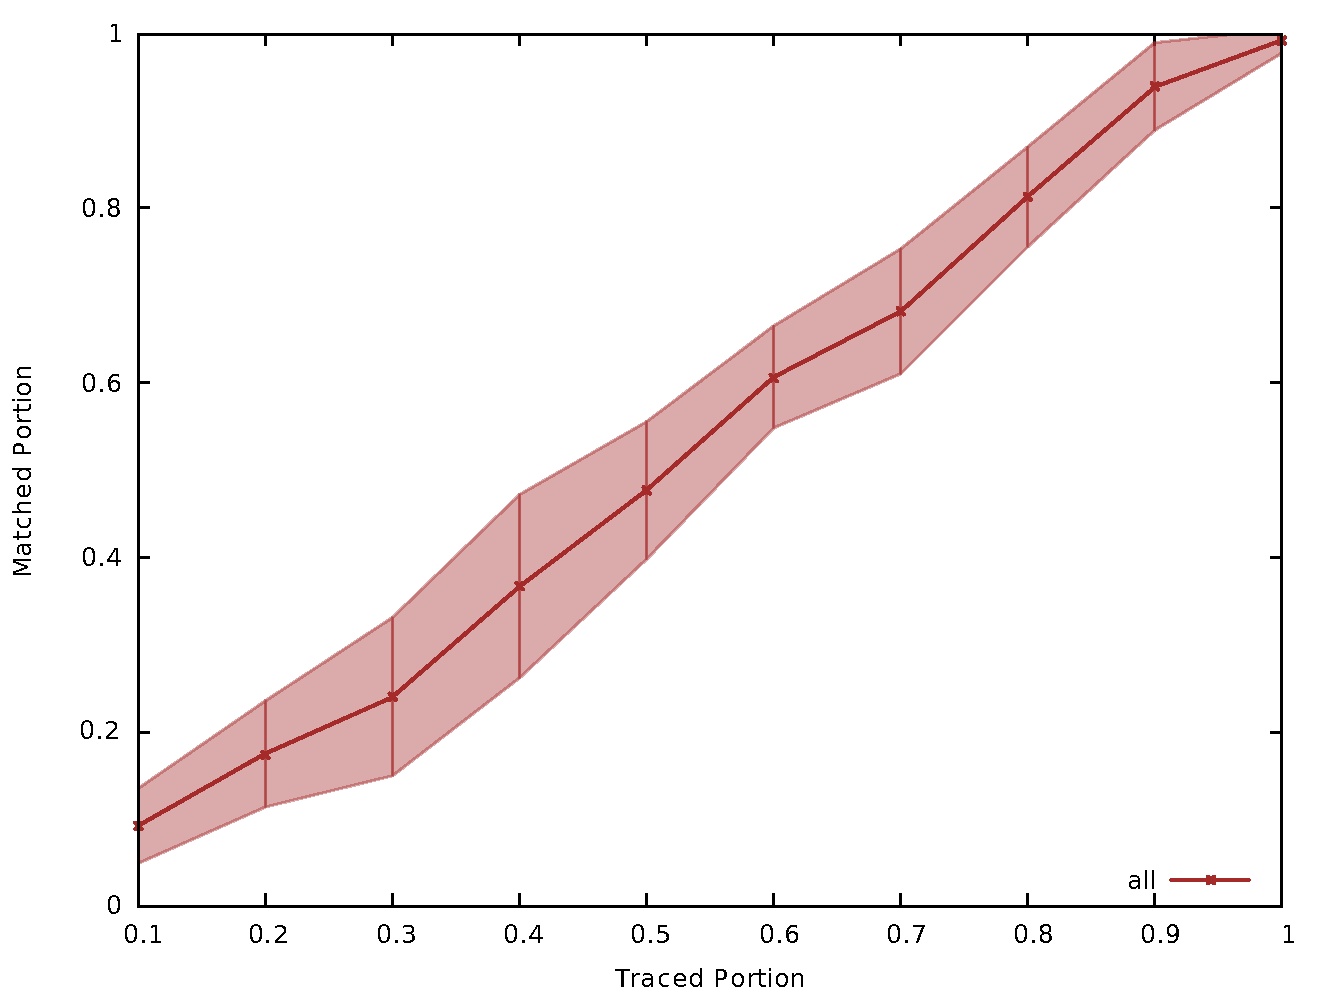
\includegraphics[width=1\linewidth]{graphs/cs_tport_mport.pdf}
		\caption{Matched portion related to the traced portion}
		\label{fig:g_tporta}
	\end{subfigure} 
	\begin{subfigure}{.5\textwidth}
		\centering
		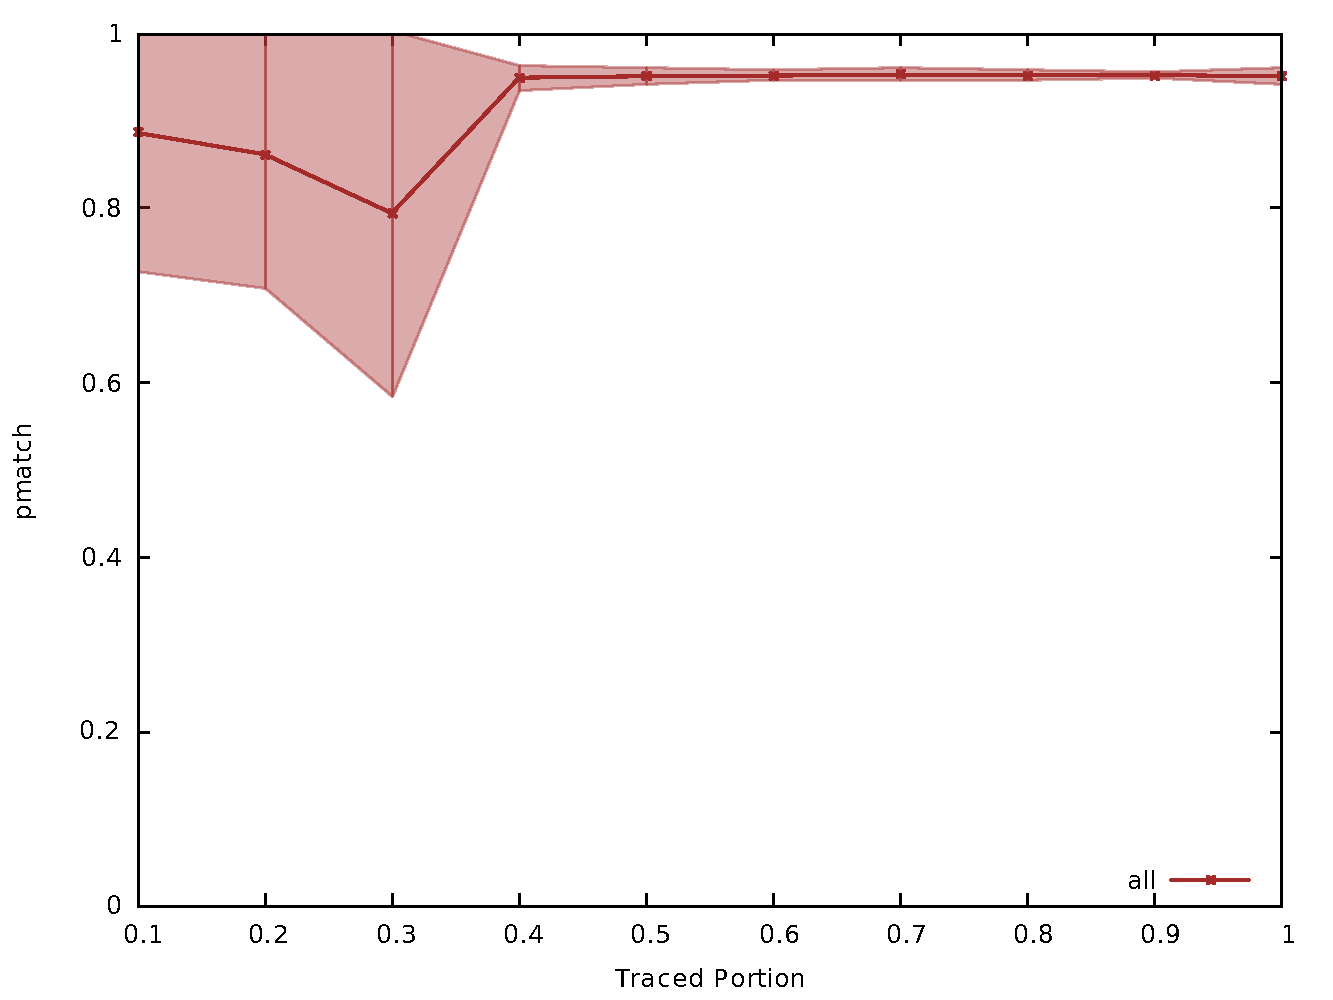
\includegraphics[width=1\linewidth]{graphs/cs_tport_pmatch.pdf}
		\caption{Matched accuracy related to the traced portion}
		\label{fig:g_tportb}
	\end{subfigure} 
	\caption{Charts about matched portion and matched accuracy at the variation of both
traced clients and traced servers}
	\label{fig:g_tport}
\end{figure}

The charts in figure \ref{fig:g_tport} show the results of the
tests where both traced servers and traced clients were variable
(variable traced portion). This
represents the most realistic scenario and we can notice that the
matched portion trend seems to respect the sum of the trend results of the other
two experiments (figure \ref{fig:g_mport}). We can see that a
time-analysis attacker should be interested to trace as much Tor
network node as possibile as the matched portion almost
linearly scales with the traced portion. As istance if an attacker is
able to trace an half of the Tor network nodes he may understand the
relations between the clients and servers of around a quarter of the Tor
network. Moreover, the matching accuracy still remains almost costant
around 1, meaning that of that quarter of the Tor network the attacker
may be able to correctly understand the end-points of almost all the connections.



\begin{figure}
	\begin{subfigure}{.5\textwidth}
		\centering
		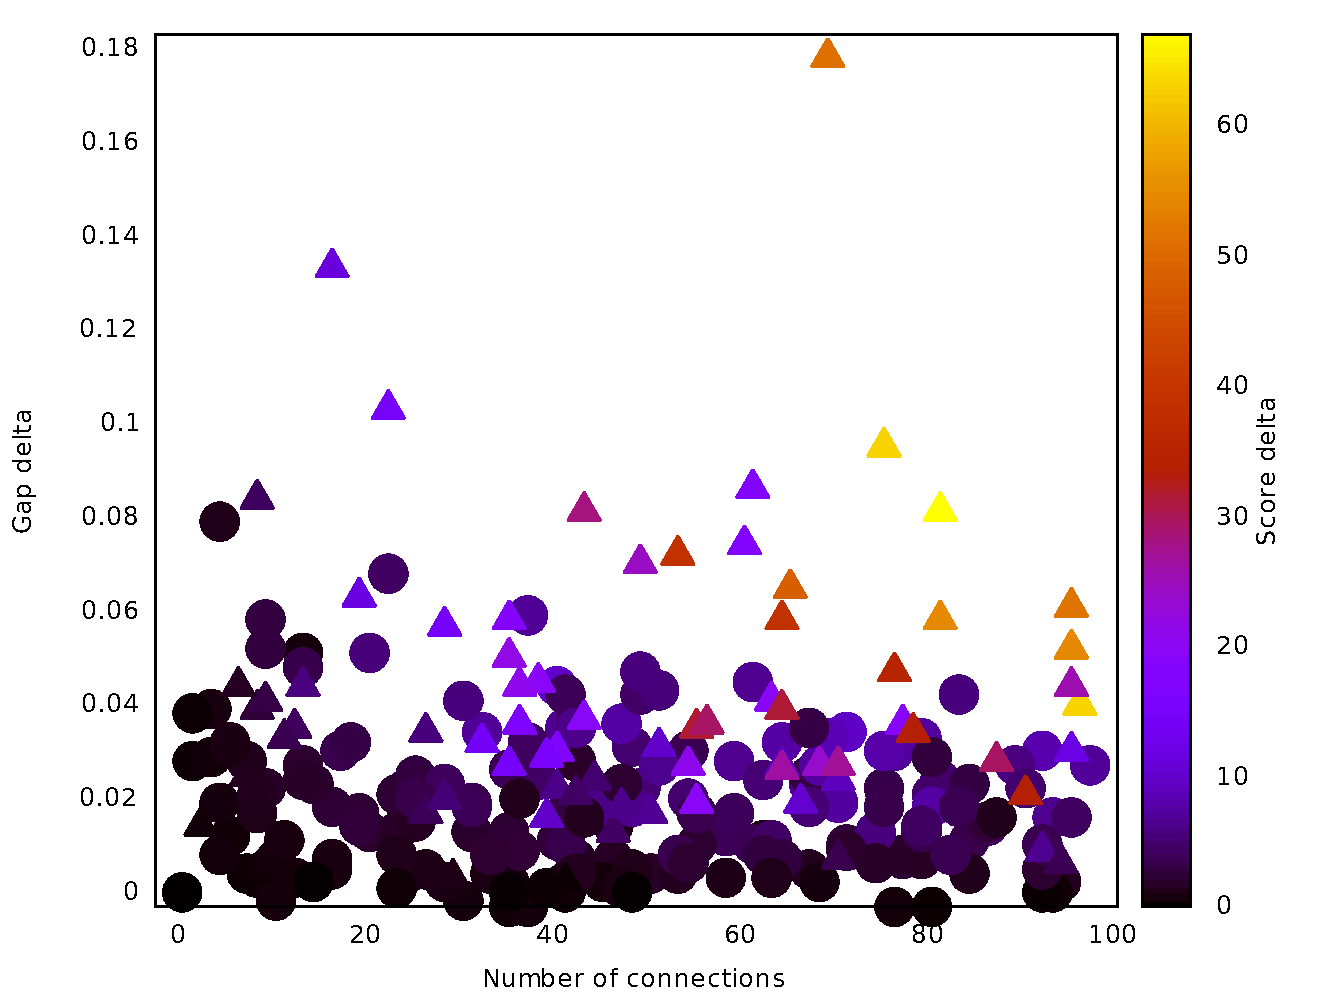
\includegraphics[width=1\linewidth]{graphs/map_cs_4_average.pdf}
		\caption{Trusted matching chart with 40\% of traced portion}
		\label{fig:g_tporta}
	\end{subfigure} 
	\begin{subfigure}{.5\textwidth}
		\centering
		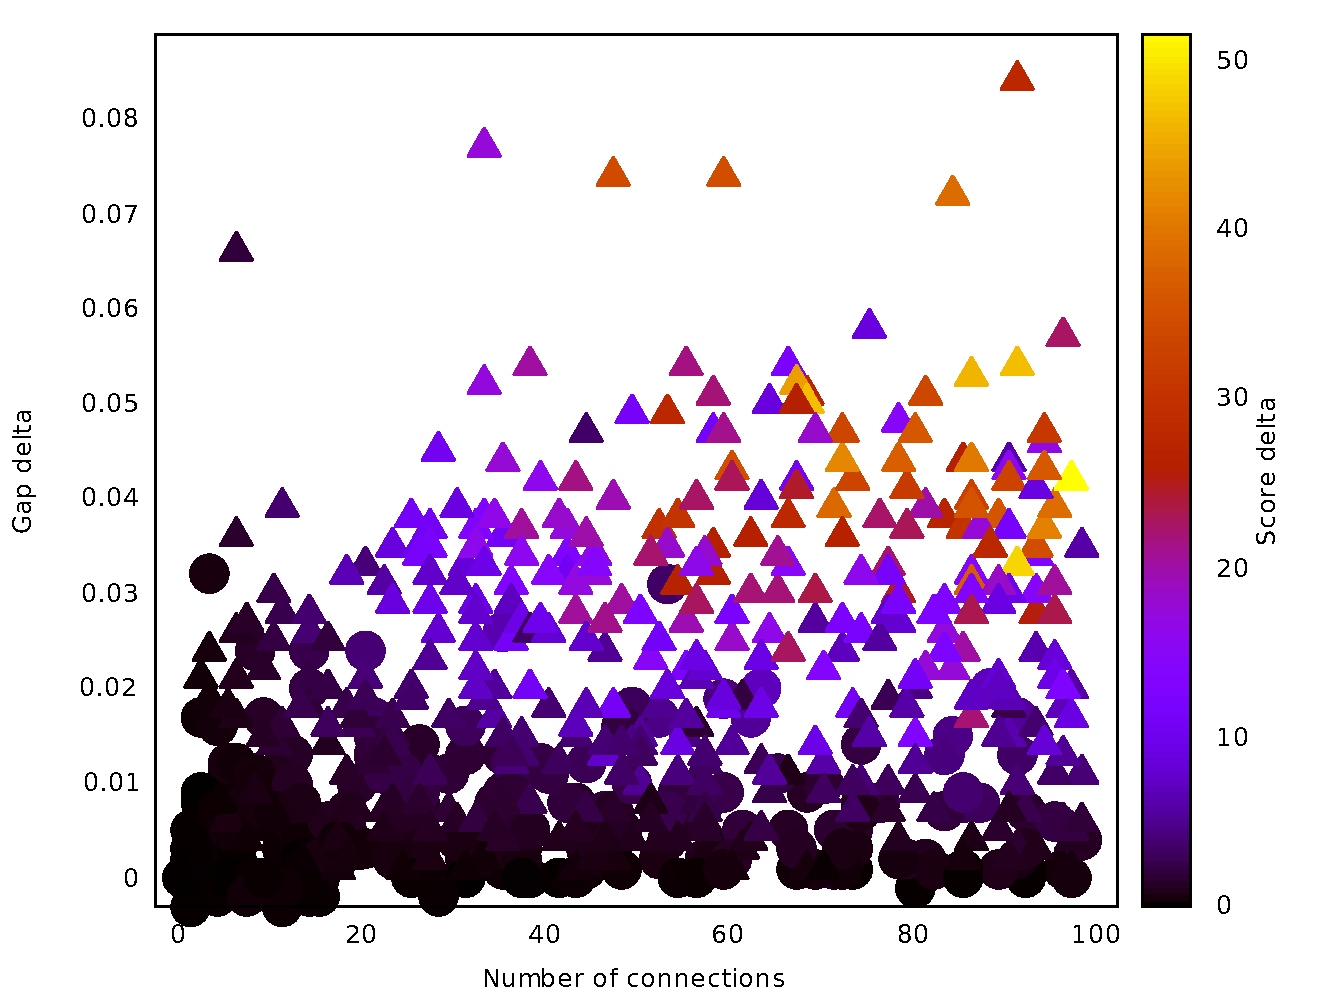
\includegraphics[width=1\linewidth]{graphs/map_cs_9_average.pdf}
		\caption{Trusted matching chart with 90\% of traced portion}
		\label{fig:g_tportb}
	\end{subfigure} 
	\caption{Charts about trusted matching parameter}
	\label{fig:g_tport}
\end{figure}


Until now we have not faced yet the problem about how an attacker can distinguish
the clients that found a right matching among the others. We based our
matching portion evaluation comparing all the results with the real
connections logged by the simulations. This is obviously not possibile
in a real scenario thus we tried to understand if an attacker may
distinguish the right matchings basing on some parameters.

\begin{figure}[H]
\centering
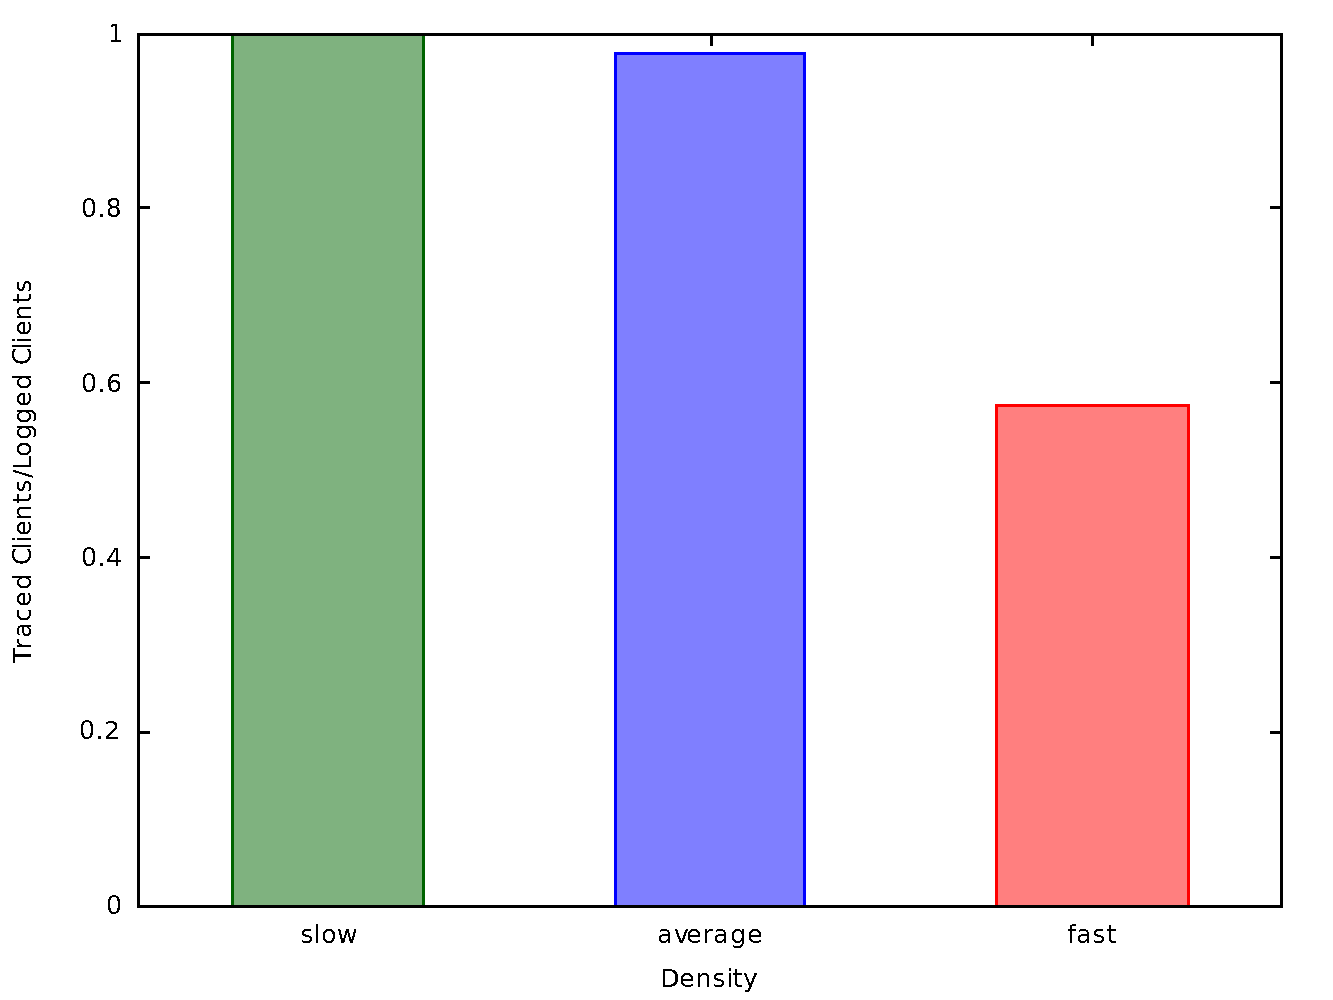
\includegraphics[scale=0.35]{graphs/density_clients_ration.pdf}
\caption{Communication density related to the logging capacity}
\label{fig:g_density}
\end{figure}

TODO BLABLABLA SU DENSITY
